% Options for packages loaded elsewhere
% Options for packages loaded elsewhere
\PassOptionsToPackage{unicode}{hyperref}
\PassOptionsToPackage{hyphens}{url}
%
\documentclass[
  ignorenonframetext,
  aspectratio=169,
  russian,
  aspectratio=169]{beamer}
\newif\ifbibliography
\usepackage{pgfpages}
\setbeamertemplate{caption}[numbered]
\setbeamertemplate{caption label separator}{: }
\setbeamercolor{caption name}{fg=normal text.fg}
\beamertemplatenavigationsymbolshorizontal
% remove section numbering
\setbeamertemplate{part page}{
  \centering
  \begin{beamercolorbox}[sep=16pt,center]{part title}
    \usebeamerfont{part title}\insertpart\par
  \end{beamercolorbox}
}
\setbeamertemplate{section page}{
  \centering
  \begin{beamercolorbox}[sep=12pt,center]{section title}
    \usebeamerfont{section title}\insertsection\par
  \end{beamercolorbox}
}
\setbeamertemplate{subsection page}{
  \centering
  \begin{beamercolorbox}[sep=8pt,center]{subsection title}
    \usebeamerfont{subsection title}\insertsubsection\par
  \end{beamercolorbox}
}
% Prevent slide breaks in the middle of a paragraph
\widowpenalties 1 10000
\raggedbottom
\AtBeginPart{
  \frame{\partpage}
}
\AtBeginSection{
  \ifbibliography
  \else
    \frame{\sectionpage}
  \fi
}
\AtBeginSubsection{
  \frame{\subsectionpage}
}
\usepackage{iftex}
\ifPDFTeX
  \usepackage[T1]{fontenc}
  \usepackage[utf8]{inputenc}
  \usepackage{textcomp} % provide euro and other symbols
\else % if luatex or xetex
  \usepackage{unicode-math} % this also loads fontspec
  \defaultfontfeatures{Scale=MatchLowercase}
  \defaultfontfeatures[\rmfamily]{Ligatures=TeX,Scale=1}
\fi
\usepackage{lmodern}

\usefonttheme{serif} % use mainfont rather than sansfont for slide text
\ifPDFTeX\else
  % xetex/luatex font selection
  \setmainfont[]{DejaVu Serif}
  \setsansfont[]{DejaVu Sans}
  \setmonofont[]{DejaVu Sans Mono}
\fi
% Use upquote if available, for straight quotes in verbatim environments
\IfFileExists{upquote.sty}{\usepackage{upquote}}{}
\IfFileExists{microtype.sty}{% use microtype if available
  \usepackage[]{microtype}
  \UseMicrotypeSet[protrusion]{basicmath} % disable protrusion for tt fonts
}{}


\usepackage{longtable,booktabs,array}
\usepackage{calc} % for calculating minipage widths
\usepackage{caption}
% Make caption package work with longtable
\makeatletter
\def\fnum@table{\tablename~\thetable}
\makeatother
\usepackage{graphicx}
\makeatletter
\newsavebox\pandoc@box
\newcommand*\pandocbounded[1]{% scales image to fit in text height/width
  \sbox\pandoc@box{#1}%
  \Gscale@div\@tempa{\textheight}{\dimexpr\ht\pandoc@box+\dp\pandoc@box\relax}%
  \Gscale@div\@tempb{\linewidth}{\wd\pandoc@box}%
  \ifdim\@tempb\p@<\@tempa\p@\let\@tempa\@tempb\fi% select the smaller of both
  \ifdim\@tempa\p@<\p@\scalebox{\@tempa}{\usebox\pandoc@box}%
  \else\usebox{\pandoc@box}%
  \fi%
}
% Set default figure placement to htbp
\def\fps@figure{htbp}
\makeatother



\ifLuaTeX
\usepackage[bidi=basic,provide=*]{babel}
\else
\usepackage[bidi=default,provide=*]{babel}
\fi
\ifPDFTeX
\else
\babelfont{rm}[]{DejaVu Serif}
\fi
% get rid of language-specific shorthands (see #6817):
\let\LanguageShortHands\languageshorthands
\def\languageshorthands#1{}


\setlength{\emergencystretch}{3em} % prevent overfull lines

\providecommand{\tightlist}{%
  \setlength{\itemsep}{0pt}\setlength{\parskip}{0pt}}



 

\usepackage[]{csquotes}

\IfFileExists{plex-otf.sty}{
  %% Full TeXlive
  % \usepackage[%
  %   % math,
  %   RM={Scale=0.94},SS={Scale=0.94},SScon={Scale=0.94},TT={Scale=MatchLowercase,FakeStretch=0.9},DefaultFeatures={Ligatures=Common}
  % ]{plex-otf}
}{
  %% TinyTeX
  \usepackage{libertine}
}

%%% Load theme
% https://deic.uab.cat/~iblanes/beamer_gallery/
\IfFileExists{beamerthemegotham.sty}{
  %% Full TeXlive
  \usetheme{gotham}
  \gothamset{
    numbering=totalpagenumber,
    parttocframe default=off,
    sectiontocframe default=off,
    subsectiontocframe default=off,
  }
}{
  %% TinyTeX
  \usetheme{Madrid}
}
\makeatletter
\@ifpackageloaded{caption}{}{\usepackage{caption}}
\AtBeginDocument{%
\ifdefined\contentsname
  \renewcommand*\contentsname{Содержание}
\else
  \newcommand\contentsname{Содержание}
\fi
\ifdefined\listfigurename
  \renewcommand*\listfigurename{Список иллюстраций}
\else
  \newcommand\listfigurename{Список иллюстраций}
\fi
\ifdefined\listtablename
  \renewcommand*\listtablename{Список таблиц}
\else
  \newcommand\listtablename{Список таблиц}
\fi
\ifdefined\figurename
  \renewcommand*\figurename{Рисунок}
\else
  \newcommand\figurename{Рисунок}
\fi
\ifdefined\tablename
  \renewcommand*\tablename{Таблица}
\else
  \newcommand\tablename{Таблица}
\fi
}
\@ifpackageloaded{float}{}{\usepackage{float}}
\floatstyle{ruled}
\@ifundefined{c@chapter}{\newfloat{codelisting}{h}{lop}}{\newfloat{codelisting}{h}{lop}[chapter]}
\floatname{codelisting}{Список}
\newcommand*\listoflistings{\listof{codelisting}{Листинги}}
\makeatother
\makeatletter
\makeatother
\makeatletter
\@ifpackageloaded{caption}{}{\usepackage{caption}}
\@ifpackageloaded{subcaption}{}{\usepackage{subcaption}}
\makeatother

\usepackage{bookmark}
\IfFileExists{xurl.sty}{\usepackage{xurl}}{} % add URL line breaks if available
\urlstyle{same}
\hypersetup{
  pdftitle={Выполнение лабораторной работы №1},
  pdfauthor={Карпухин Клим},
  pdflang={ru-RU},
  hidelinks,
  pdfcreator={LaTeX via pandoc}}


\title{Выполнение лабораторной работы №1}
\subtitle{Установка ОС Linux}
\author{Карпухин Клим}
\date{2026-03-01}

\begin{document}
\frame{\titlepage}


\section{Содержание}\label{ux441ux43eux434ux435ux440ux436ux430ux43dux438ux435}

\begin{frame}{Содержание}
\begin{enumerate}[<+->]
\tightlist
\item
  Информация о докладчике
\item
  Вводная часть и актуальность
\item
  Объект и предмет исследования
\item
  Цель, гипотеза, задачи
\item
  Материалы, методы и инструменты
\item
  Ход работы (этапы, скриншоты)
\item
  Результаты и анализ
\item
  Выводы
\item
  Контрольные вопросы
\item
  Список литературы
\end{enumerate}
\end{frame}

\section{Информация}\label{ux438ux43dux444ux43eux440ux43cux430ux446ux438ux44f}

\begin{frame}{Докладчик}
\phantomsection\label{ux434ux43eux43aux43bux430ux434ux447ux438ux43a}
\begin{columns}[c]
\begin{column}{0.65\linewidth}
\begin{itemize}[<+->]
\tightlist
\item
  \textbf{Карпухин Клим}
\item
  Российский университет дружбы народов
\item
  Email:
  \href{mailto:1032255580@rudn.ru}{\nolinkurl{1032255580@rudn.ru}}
\item
  Роли: студент (лабораторная работа по ОС/виртуализации)
\end{itemize}
\end{column}

\begin{column}{0.35\linewidth}

\includegraphics[width=0.9\linewidth,height=\textheight,keepaspectratio]{./image/dokladchik.png}
\end{column}
\end{columns}
\end{frame}

\section{Вводная
часть}\label{ux432ux432ux43eux434ux43dux430ux44f-ux447ux430ux441ux442ux44c}

\begin{frame}{Актуальность}
\phantomsection\label{ux430ux43aux442ux443ux430ux43bux44cux43dux43eux441ux442ux44c}
\begin{itemize}[<+->]
\tightlist
\item
  Практические навыки установки и конфигурирования Linux необходимы для
  изучения системного администрирования и разработки.
\item
  Виртуальные машины позволяют безопасно экспериментировать с ОС, не
  рискуя основной системой.
\end{itemize}
\end{frame}

\begin{frame}{Объект и предмет исследования}
\phantomsection\label{ux43eux431ux44aux435ux43aux442-ux438-ux43fux440ux435ux434ux43cux435ux442-ux438ux441ux441ux43bux435ux434ux43eux432ux430ux43dux438ux44f}
\begin{itemize}[<+->]
\tightlist
\item
  \textbf{Объект:} виртуальная машина с установленной ОС Linux.
\item
  \textbf{Предмет:} процесс установки ОС Fedora (Sway), базовая
  конфигурация и получение системной информации.
\end{itemize}
\end{frame}

\section{Научная новизна и практическая
значимость}\label{ux43dux430ux443ux447ux43dux430ux44f-ux43dux43eux432ux438ux437ux43dux430-ux438-ux43fux440ux430ux43aux442ux438ux447ux435ux441ux43aux430ux44f-ux437ux43dux430ux447ux438ux43cux43eux441ux442ux44c}

\begin{frame}{Научная новизна}
\phantomsection\label{ux43dux430ux443ux447ux43dux430ux44f-ux43dux43eux432ux438ux437ux43dux430}
\begin{itemize}[<+->]
\tightlist
\item
  Демонстрация практической последовательности установки и конфигурации
  минимального рабочего окружения (Sway) и автоматизации обновлений в
  виртуальной среде.
\end{itemize}
\end{frame}

\begin{frame}{Практическая значимость}
\phantomsection\label{ux43fux440ux430ux43aux442ux438ux447ux435ux441ux43aux430ux44f-ux437ux43dux430ux447ux438ux43cux43eux441ux442ux44c}
\begin{itemize}[<+->]
\tightlist
\item
  Полученные навыки пригодны для развертывания тестовых сред,
  преподавания лабораторных работ и подготовки документации (pandoc +
  TeX Live).
\end{itemize}
\end{frame}

\section{Цель, гипотеза и
задачи}\label{ux446ux435ux43bux44c-ux433ux438ux43fux43eux442ux435ux437ux430-ux438-ux437ux430ux434ux430ux447ux438}

\begin{frame}{Цель}
\phantomsection\label{ux446ux435ux43bux44c}
Приобрести практические навыки установки и базовой настройки ОС Linux на
виртуальной машине.
\end{frame}

\begin{frame}{Гипотеза}
\phantomsection\label{ux433ux438ux43fux43eux442ux435ux437ux430}
Правильная настройка виртуальной машины и минимальный набор системных
пакетов обеспечат рабочее окружение, пригодное для дальнейших
лабораторных и исследовательских работ.
\end{frame}

\begin{frame}{Задачи}
\phantomsection\label{ux437ux430ux434ux430ux447ux438}
\begin{itemize}[<+->]
\tightlist
\item
  Создать виртуальную машину (VirtualBox/QEMU).
\item
  Установить Fedora (Sway).
\item
  Настроить базовые сервисы, автоматические обновления, отключить
  SELinux (по заданию).
\item
  Получить и зафиксировать системную информацию (ядро, CPU, память, FS,
  гипервизор).
\end{itemize}
\end{frame}

\section{Материалы и
методы}\label{ux43cux430ux442ux435ux440ux438ux430ux43bux44b-ux438-ux43cux435ux442ux43eux434ux44b}

\begin{frame}[fragile]{Оборудование / ПО}
\phantomsection\label{ux43eux431ux43eux440ux443ux434ux43eux432ux430ux43dux438ux435-ux43fux43e}
\begin{itemize}[<+->]
\tightlist
\item
  Hypervisor: VirtualBox (гипервизор второго типа).
\item
  Дистрибутив: Fedora (вариант Sway).
\item
  Утилиты и инструменты: \texttt{dnf}, \texttt{systemd}, \texttt{tmux},
  \texttt{pandoc}, \texttt{TeX\ Live}.
\end{itemize}
\end{frame}

\section{Ход работы --- подготовка виртуальной машины
(этапы)}\label{ux445ux43eux434-ux440ux430ux431ux43eux442ux44b-ux43fux43eux434ux433ux43eux442ux43eux432ux43aux430-ux432ux438ux440ux442ux443ux430ux43bux44cux43dux43eux439-ux43cux430ux448ux438ux43dux44b-ux44dux442ux430ux43fux44b}

\begin{frame}{Подготовка виртуальной машины (1)}
\phantomsection\label{ux43fux43eux434ux433ux43eux442ux43eux432ux43aux430-ux432ux438ux440ux442ux443ux430ux43bux44cux43dux43eux439-ux43cux430ux448ux438ux43dux44b-1}
\begin{enumerate}[<+->]
\tightlist
\item
  Создание VM в GUI VirtualBox (указано имя согласно логину).
  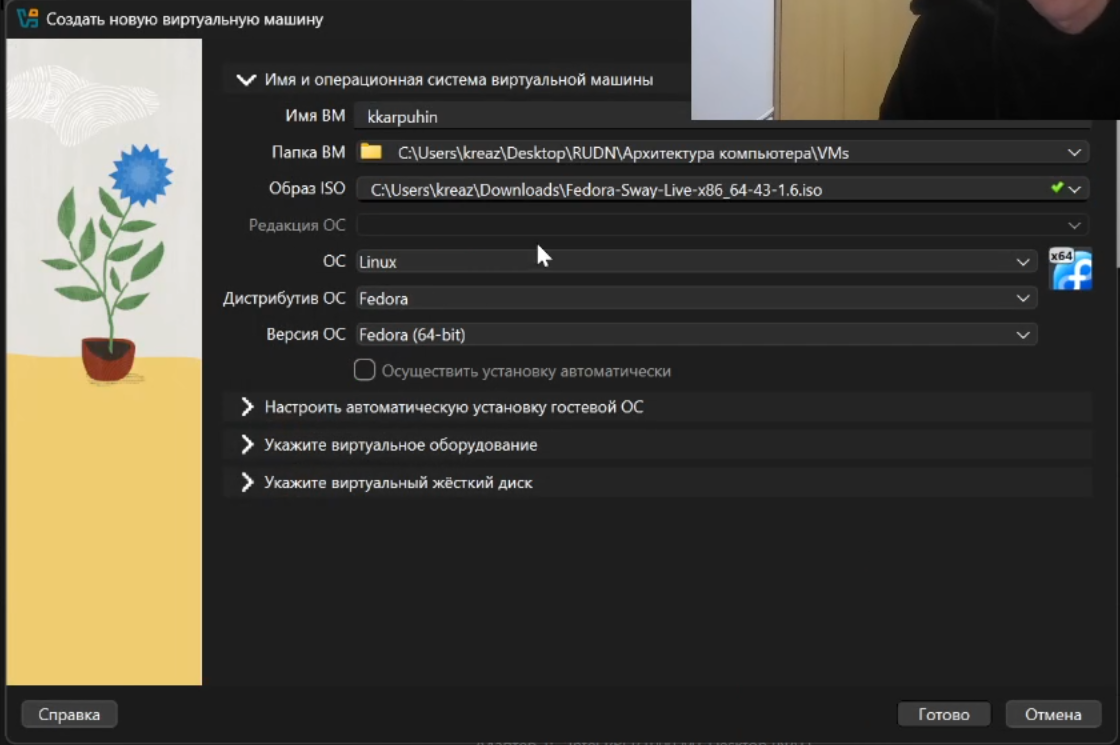
\includegraphics[width=0.3\linewidth,height=\textheight,keepaspectratio]{image/1.png}
\end{enumerate}
\end{frame}

\begin{frame}{Подготовка виртуальной машины (2)}
\phantomsection\label{ux43fux43eux434ux433ux43eux442ux43eux432ux43aux430-ux432ux438ux440ux442ux443ux430ux43bux44cux43dux43eux439-ux43cux430ux448ux438ux43dux44b-2}
\begin{enumerate}[<+->]
\setcounter{enumi}{1}
\tightlist
\item
  Указание объёма RAM --- 6107 МБ.
  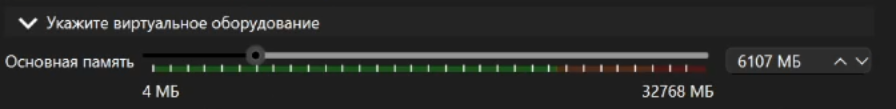
\includegraphics[width=0.3\linewidth,height=\textheight,keepaspectratio]{image/2.png}
\end{enumerate}
\end{frame}

\begin{frame}{Подготовка виртуальной машины (3)}
\phantomsection\label{ux43fux43eux434ux433ux43eux442ux43eux432ux43aux430-ux432ux438ux440ux442ux443ux430ux43bux44cux43dux43eux439-ux43cux430ux448ux438ux43dux44b-3}
\begin{enumerate}[<+->]
\setcounter{enumi}{2}
\tightlist
\item
  Размер виртуального диска --- 80 ГБ.
  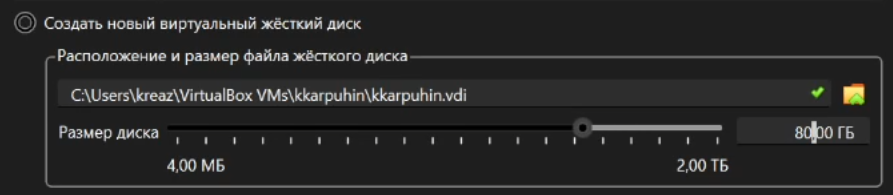
\includegraphics[width=0.3\linewidth,height=\textheight,keepaspectratio]{image/3.png}
\end{enumerate}
\end{frame}

\begin{frame}{Подготовка виртуальной машины (4)}
\phantomsection\label{ux43fux43eux434ux433ux43eux442ux43eux432ux43aux430-ux432ux438ux440ux442ux443ux430ux43bux44cux43dux43eux439-ux43cux430ux448ux438ux43dux44b-4}
\begin{enumerate}[<+->]
\setcounter{enumi}{3}
\tightlist
\item
  Графический контроллер --- VMSVGA; включено 3D-ускорение.
  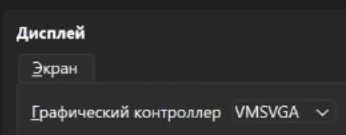
\includegraphics[width=0.2\linewidth,height=\textheight,keepaspectratio]{image/4.png}
  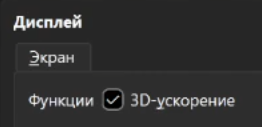
\includegraphics[width=0.2\linewidth,height=\textheight,keepaspectratio]{image/5.png}
\end{enumerate}
\end{frame}

\begin{frame}{Подготовка виртуальной машины (5)}
\phantomsection\label{ux43fux43eux434ux433ux43eux442ux43eux432ux43aux430-ux432ux438ux440ux442ux443ux430ux43bux44cux43dux43eux439-ux43cux430ux448ux438ux43dux44b-5}
\begin{enumerate}[<+->]
\setcounter{enumi}{4}
\tightlist
\item
  Включены общий буфер обмена и drag'n'drop.
  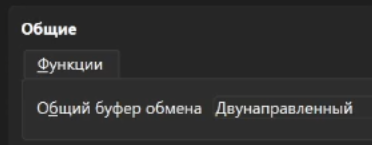
\includegraphics[width=0.3\linewidth,height=\textheight,keepaspectratio]{image/6.png}
\end{enumerate}
\end{frame}

\begin{frame}{Подготовка виртуальной машины (6)}
\phantomsection\label{ux43fux43eux434ux433ux43eux442ux43eux432ux43aux430-ux432ux438ux440ux442ux443ux430ux43bux44cux43dux43eux439-ux43cux430ux448ux438ux43dux44b-6}
\begin{enumerate}[<+->]
\setcounter{enumi}{5}
\tightlist
\item
  Включена поддержка UEFI.
  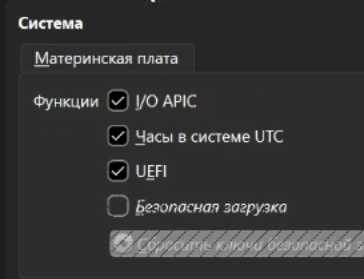
\includegraphics[width=0.3\linewidth,height=\textheight,keepaspectratio]{image/7.png}
\end{enumerate}
\end{frame}

\section{Ход работы --- установка и базовая
настройка}\label{ux445ux43eux434-ux440ux430ux431ux43eux442ux44b-ux443ux441ux442ux430ux43dux43eux432ux43aux430-ux438-ux431ux430ux437ux43eux432ux430ux44f-ux43dux430ux441ux442ux440ux43eux439ux43aux430}

\begin{frame}{Установка и базовая настройка (1)}
\phantomsection\label{ux443ux441ux442ux430ux43dux43eux432ux43aux430-ux438-ux431ux430ux437ux43eux432ux430ux44f-ux43dux430ux441ux442ux440ux43eux439ux43aux430-1}
\begin{enumerate}[<+->]
\tightlist
\item
  Установка системы с Live-ISO, разметка диска, ввод пользовательских
  данных, установка загрузчика.
  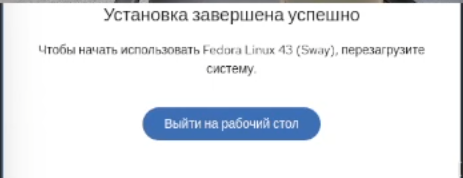
\includegraphics[width=0.3\linewidth,height=\textheight,keepaspectratio]{image/8.png}
\end{enumerate}
\end{frame}

\begin{frame}{Установка и базовая настройка (2)}
\phantomsection\label{ux443ux441ux442ux430ux43dux43eux432ux43aux430-ux438-ux431ux430ux437ux43eux432ux430ux44f-ux43dux430ux441ux442ux440ux43eux439ux43aux430-2}
\begin{enumerate}[<+->]
\setcounter{enumi}{1}
\tightlist
\item
  Переключение на root и установка средств разработки.
  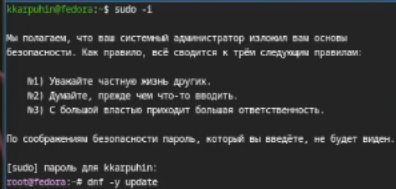
\includegraphics[width=0.3\linewidth,height=\textheight,keepaspectratio]{image/9.png}
\end{enumerate}
\end{frame}

\begin{frame}[fragile]{Установка и базовая настройка (3)}
\phantomsection\label{ux443ux441ux442ux430ux43dux43eux432ux43aux430-ux438-ux431ux430ux437ux43eux432ux430ux44f-ux43dux430ux441ux442ux440ux43eux439ux43aux430-3}
\begin{enumerate}[<+->]
\setcounter{enumi}{2}
\tightlist
\item
  Обновление пакетов (\texttt{dnf\ update}).
  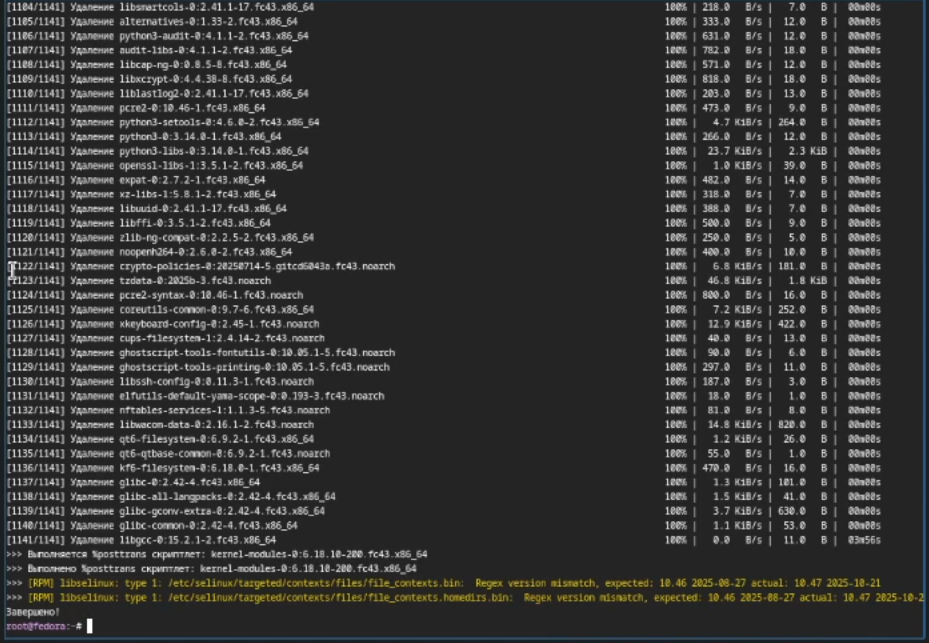
\includegraphics[width=0.3\linewidth,height=\textheight,keepaspectratio]{image/10.png}
\end{enumerate}
\end{frame}

\begin{frame}{Установка и базовая настройка (4)}
\phantomsection\label{ux443ux441ux442ux430ux43dux43eux432ux43aux430-ux438-ux431ux430ux437ux43eux432ux430ux44f-ux43dux430ux441ux442ux440ux43eux439ux43aux430-4}
\begin{enumerate}[<+->]
\setcounter{enumi}{3}
\tightlist
\item
  Установка удобных утилит для терминала.
  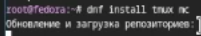
\includegraphics[width=0.3\linewidth,height=\textheight,keepaspectratio]{image/11.png}
\end{enumerate}
\end{frame}

\begin{frame}[fragile]{Установка и базовая настройка (5)}
\phantomsection\label{ux443ux441ux442ux430ux43dux43eux432ux43aux430-ux438-ux431ux430ux437ux43eux432ux430ux44f-ux43dux430ux441ux442ux440ux43eux439ux43aux430-5}
\begin{enumerate}[<+->]
\setcounter{enumi}{4}
\tightlist
\item
  Установка и запуск \texttt{dnf-automatic} - автоматические обновления.
  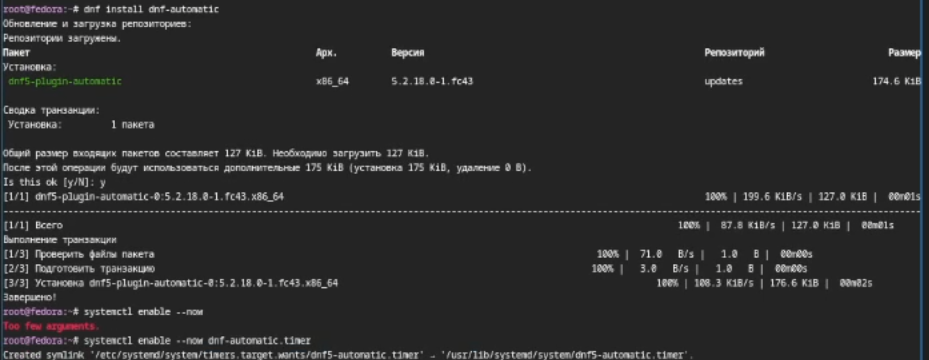
\includegraphics[width=0.3\linewidth,height=\textheight,keepaspectratio]{image/12.png}
\end{enumerate}
\end{frame}

\begin{frame}{Установка и базовая настройка (6)}
\phantomsection\label{ux443ux441ux442ux430ux43dux43eux432ux43aux430-ux438-ux431ux430ux437ux43eux432ux430ux44f-ux43dux430ux441ux442ux440ux43eux439ux43aux430-6}
\begin{enumerate}[<+->]
\setcounter{enumi}{5}
\tightlist
\item
  Отключение SELinux.
  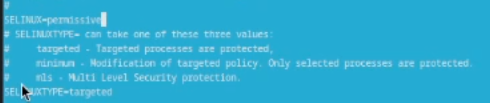
\includegraphics[width=0.3\linewidth,height=\textheight,keepaspectratio]{image/13.png}
\end{enumerate}
\end{frame}

\section{Ход работы --- конфигурация рабочего
окружения}\label{ux445ux43eux434-ux440ux430ux431ux43eux442ux44b-ux43aux43eux43dux444ux438ux433ux443ux440ux430ux446ux438ux44f-ux440ux430ux431ux43eux447ux435ux433ux43e-ux43eux43aux440ux443ux436ux435ux43dux438ux44f}

\begin{frame}[fragile]{Конфигурация рабочего окружения (1)}
\phantomsection\label{ux43aux43eux43dux444ux438ux433ux443ux440ux430ux446ux438ux44f-ux440ux430ux431ux43eux447ux435ux433ux43e-ux43eux43aux440ux443ux436ux435ux43dux438ux44f-1}
\begin{itemize}[<+->]
\tightlist
\item
  Запуск \texttt{tmux} для удобства работы в терминале.
  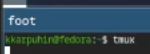
\includegraphics[width=0.3\linewidth,height=\textheight,keepaspectratio]{image/14.png}
\end{itemize}
\end{frame}

\begin{frame}{Конфигурация рабочего окружения (2)}
\phantomsection\label{ux43aux43eux43dux444ux438ux433ux443ux440ux430ux446ux438ux44f-ux440ux430ux431ux43eux447ux435ux433ux43e-ux43eux43aux440ux443ux436ux435ux43dux438ux44f-2}
\begin{itemize}[<+->]
\tightlist
\item
  Создание и редактирование конфигурации Sway:
  `\textasciitilde/.config/sway/config.d/95-system-keyboard-config.conf.
  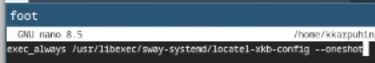
\includegraphics[width=0.3\linewidth,height=\textheight,keepaspectratio]{image/15.png}
\end{itemize}
\end{frame}

\begin{frame}{Конфигурация рабочего окружения (3)}
\phantomsection\label{ux43aux43eux43dux444ux438ux433ux443ux440ux430ux446ux438ux44f-ux440ux430ux431ux43eux447ux435ux433ux43e-ux43eux43aux440ux443ux436ux435ux43dux438ux44f-3}
\begin{itemize}[<+->]
\tightlist
\item
  Редактирование конфигураций от root (привилегии).
  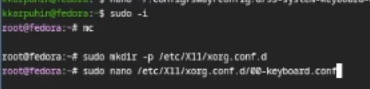
\includegraphics[width=0.7\linewidth,height=\textheight,keepaspectratio]{image/16.png}
\end{itemize}
\end{frame}

\begin{frame}{Конфигурация рабочего окружения (4)}
\phantomsection\label{ux43aux43eux43dux444ux438ux433ux443ux440ux430ux446ux438ux44f-ux440ux430ux431ux43eux447ux435ux433ux43e-ux43eux43aux440ux443ux436ux435ux43dux438ux44f-4}
\begin{figure}

\centering{

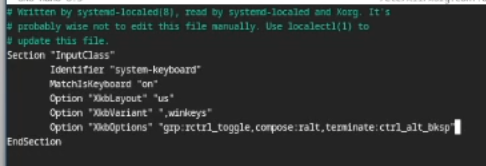
\includegraphics[width=0.3\linewidth,height=\textheight,keepaspectratio]{image/17.png}

}

\caption{\label{fig-017}Отредактированный конфигурационный файл}

\end{figure}%
\end{frame}

\begin{frame}{Конфигурация рабочего окружения (5)}
\phantomsection\label{ux43aux43eux43dux444ux438ux433ux443ux440ux430ux446ux438ux44f-ux440ux430ux431ux43eux447ux435ux433ux43e-ux43eux43aux440ux443ux436ux435ux43dux438ux44f-5}
\begin{itemize}[<+->]
\tightlist
\item
  Установка имени хоста и проверка.
  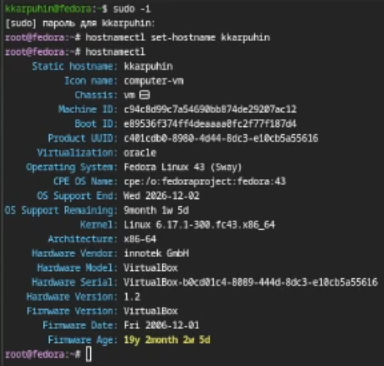
\includegraphics[width=0.3\linewidth,height=\textheight,keepaspectratio]{image/18.png}
\end{itemize}
\end{frame}

\section{Документация и подготовка
отчёта}\label{ux434ux43eux43aux443ux43cux435ux43dux442ux430ux446ux438ux44f-ux438-ux43fux43eux434ux433ux43eux442ux43eux432ux43aux430-ux43eux442ux447ux451ux442ux430}

\begin{frame}[fragile]{Документация и подготовка отчёта}
\begin{itemize}[<+->]
\tightlist
\item
  Установка \texttt{pandoc} для подготовки отчёта в Markdown → PDF/HTML.
  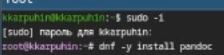
\includegraphics[width=0.3\linewidth,height=\textheight,keepaspectratio]{image/19.png}
\item
  Установка TeX Live для сборки PDF через LaTeX. !{[}Установка TeX
  Live{]}
\end{itemize}
\end{frame}

\section{Домашнее задание --- полученные системные
данные}\label{ux434ux43eux43cux430ux448ux43dux435ux435-ux437ux430ux434ux430ux43dux438ux435-ux43fux43eux43bux443ux447ux435ux43dux43dux44bux435-ux441ux438ux441ux442ux435ux43cux43dux44bux435-ux434ux430ux43dux43dux44bux435}

\begin{frame}{Домашнее задание (1)}
\phantomsection\label{ux434ux43eux43cux430ux448ux43dux435ux435-ux437ux430ux434ux430ux43dux438ux435-1}
\begin{itemize}[<+->]
\tightlist
\item
  Версия ядра Linux.
  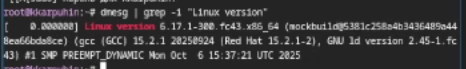
\includegraphics[width=0.3\linewidth,height=\textheight,keepaspectratio]{image/21.png}
\item
  Частота процессора.
  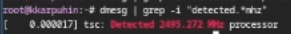
\includegraphics[width=0.3\linewidth,height=\textheight,keepaspectratio]{image/22.png}
\end{itemize}
\end{frame}

\begin{frame}{Домашнее задание (2)}
\phantomsection\label{ux434ux43eux43cux430ux448ux43dux435ux435-ux437ux430ux434ux430ux43dux438ux435-2}
\begin{itemize}[<+->]
\tightlist
\item
  Модель процессора.
  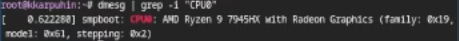
\includegraphics[width=0.3\linewidth,height=\textheight,keepaspectratio]{image/23.png}
\item
  Тип обнаруженного гипервизора.
  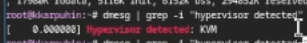
\includegraphics[width=0.3\linewidth,height=\textheight,keepaspectratio]{image/24.png}
\end{itemize}
\end{frame}

\begin{frame}{Домашнее задание (3)}
\phantomsection\label{ux434ux43eux43cux430ux448ux43dux435ux435-ux437ux430ux434ux430ux43dux438ux435-3}
\begin{itemize}[<+->]
\tightlist
\item
  Тип файловой системы корня.
  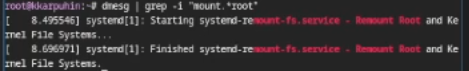
\includegraphics[width=0.3\linewidth,height=\textheight,keepaspectratio]{image/25.png}
\item
  Доступная оперативная память.
  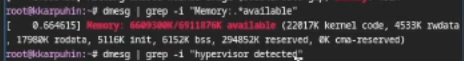
\includegraphics[width=0.3\linewidth,height=\textheight,keepaspectratio]{image/26.png}
\item
  Последовательность монтирования файловых систем.
  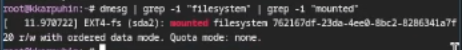
\includegraphics[width=0.3\linewidth,height=\textheight,keepaspectratio]{image/27.png}
\end{itemize}
\end{frame}

\section{Анализ и практическая значимость
результатов}\label{ux430ux43dux430ux43bux438ux437-ux438-ux43fux440ux430ux43aux442ux438ux447ux435ux441ux43aux430ux44f-ux437ux43dux430ux447ux438ux43cux43eux441ux442ux44c-ux440ux435ux437ux443ux43bux44cux442ux430ux442ux43eux432}

\begin{frame}{Анализ и практическая значимость результатов}
\begin{itemize}[<+->]
\tightlist
\item
  Установка и базовая настройка выполнены последовательно: VM → ОС →
  пакеты → конфигурация.
\item
  Автоматизация обновлений и установка инструментов разработки делают
  систему готовой к дальнейшим лабораторным.
\item
  Полученная системная информация позволяет документировать и
  воспроизвести окружение.
\end{itemize}
\end{frame}

\section{Выводы (общее
заключение)}\label{ux432ux44bux432ux43eux434ux44b-ux43eux431ux449ux435ux435-ux437ux430ux43aux43bux44eux447ux435ux43dux438ux435}

\begin{frame}{Выводы (общее заключение)}
\begin{itemize}[<+->]
\tightlist
\item
  Освоены базовые приёмы установки и конфигурации Linux в виртуальной
  машине.
\item
  Научились получать и фиксировать ключевые данные о системе (ядро, CPU,
  FS, гипервизор, память).
\item
  Отчёт оформлен в Markdown; результат может быть экспортирован в
  PDF/HTML с помощью pandoc и TeX Live.
\end{itemize}
\end{frame}

\section{Контрольные
вопросы}\label{ux43aux43eux43dux442ux440ux43eux43bux44cux43dux44bux435-ux432ux43eux43fux440ux43eux441ux44b}

\begin{frame}[fragile]{Контрольные вопросы (1)}
\phantomsection\label{ux43aux43eux43dux442ux440ux43eux43bux44cux43dux44bux435-ux432ux43eux43fux440ux43eux441ux44b-1}
\begin{enumerate}[<+->]
\item
  Информация учётной записи пользователя:

  \begin{itemize}[<+->]
  \tightlist
  \item
    Системное имя; UID; GID; полное имя; домашний каталог; начальная
    оболочка.
  \end{itemize}
\item
  Примеры команд:

  \begin{itemize}[<+->]
  \tightlist
  \item
    Справка: \texttt{-\/-help} (пример: \texttt{ls\ -\/-help})
  \item
    Текущий путь: \texttt{pwd}
  \item
    Смена каталога: \texttt{cd}, \texttt{cd\ ..},
    \texttt{cd\ \textasciitilde{}}
  \item
    Просмотр: \texttt{ls}, \texttt{ls\ -la}
  \item
    Размер каталога: \texttt{du\ -sh}
  \item
    Создать каталог/файл: \texttt{mkdir}, \texttt{touch}
  \item
    Удаление: \texttt{rmdir} (пустой), \texttt{rm\ -r} (с содержимым),
    \texttt{rm} (файл)
  \item
    Права: \texttt{chmod}, \texttt{chown}
  \item
    История: \texttt{history}
  \end{itemize}
\end{enumerate}
\end{frame}

\begin{frame}[fragile]{Контрольные вопросы (2)}
\phantomsection\label{ux43aux43eux43dux442ux440ux43eux43bux44cux43dux44bux435-ux432ux43eux43fux440ux43eux441ux44b-2}
\begin{enumerate}[<+->]
\setcounter{enumi}{2}
\item
  Файловые системы:

  \begin{itemize}[<+->]
  \tightlist
  \item
    \texttt{ext4}, \texttt{xfs}, \texttt{btrfs}, \texttt{vfat},
    \texttt{ntfs}.
  \end{itemize}
\item
  Просмотр смонтированных ФС:

  \begin{itemize}[<+->]
  \tightlist
  \item
    \texttt{mount}, \texttt{findmnt}, \texttt{df\ -T},
    \texttt{cat\ /proc/mounts}.
  \end{itemize}
\item
  Удаление зависшего процесса:

  \begin{itemize}[<+->]
  \tightlist
  \item
    Поиск:
    \texttt{ps\ aux\ \textbar{}\ grep\ \textless{}name\textgreater{}},
    \texttt{top}
  \item
    Остановка: \texttt{kill\ \textless{}PID\textgreater{}}
  \end{itemize}
\end{enumerate}
\end{frame}

\section{Рекомендации по продолжению
работы}\label{ux440ux435ux43aux43eux43cux435ux43dux434ux430ux446ux438ux438-ux43fux43e-ux43fux440ux43eux434ux43eux43bux436ux435ux43dux438ux44e-ux440ux430ux431ux43eux442ux44b}

\begin{frame}{Рекомендации по продолжению работы}
\begin{itemize}[<+->]
\tightlist
\item
  Откатить отключение SELinux только при наличии обоснования, по
  умолчанию SELinux рекомендуется держать включённым.
\item
  Настроить бэкап/снапшоты виртуальной машины перед экспериментами.
\item
  Внедрить управление конфигурацией (Ansible) для повторяемости
  настроек.
\end{itemize}
\end{frame}




\end{document}
